\documentclass[a4paper]{article}
\usepackage{subfigure}
\usepackage{amsmath,amssymb,algorithmic,booktabs,bm,caption,cases,csvsimple,enumerate,float,geometry,graphicx,indentfirst,listings,makecell,multirow,setspace,tabularx,titlesec,xcolor}
\geometry{left=3.5cm,right=3.5cm,top=3.3cm,bottom=3.3cm}
\lstset{
	language=Matlab, numbers=left, tabsize=4,
	framexleftmargin=1.5mm, frame=leftline,
	keywordstyle=\color{blue}\bfseries,
	identifierstyle=\bf, breaklines=true, 
	basicstyle=\normalsize,rulecolor=\color{brown}, 
	numberstyle=\color[RGB]{20,20,20}
}
\begin{document}
\begin{titlepage}
	\begin{Large}
		\begin{center}
			\noindent\rule[0.25\baselineskip]{\textwidth}{1pt}
			\vspace{0.5cm}
			\textsc{UM--SJTU Joint Institute}\\
			\vspace{0.25cm}
			\textsc{Signals and Systems\\(VE216)}
			\noindent\rule[0.25\baselineskip]{\textwidth}{1pt}
			\vspace{4.9cm}\\
			\textsc{Laboratory Report}\\
			\vspace{0.85cm}
			\textsc{Lab 1}\\
			\vspace{0.5em}
			LTI Systems
			\vspace{6cm}
		\end{center}
	\end{Large}
	\begin{tabular}{ll}
		Name: Yihua Liu&ID:518021910998\\
		&\\
		Date: \today&\\
	\end{tabular}
\end{titlepage}
\newpage
\renewcommand\thesection{\arabic{section}}
\section{Objectives}
\begin{itemize}
	\item To become familiar with the laboratory equipment: power supply, signal generator, digital oscilloscope, computer data acquisition system (Scope Connect).
	\item To review basic concepts of linear time-invariant systems.
	\item To illustrate several possible ways to determine the impulse response of a physical system from measured data.
	\item To use linearity, time-invariance and impulse response to compute the output of an LTI system when the input is a step, a pulse, or a more complicated signal. You will compare these calculations with actual measurements.
	\item To measure the frequency response of an LTI system and compare against theory.
	\item Measure the output response of the series RC circuit for a variety of inputs, including a step, a combination of a step and a ramp, and a sinusoid.
	\item Compare results to those computed as part of pre-lab assignment.
\end{itemize}
\section{Theoretical background}
An RC circuit is used so that the computations are easy and physically meaningful. The same procedures can be applied to much more complicated systems.
\subsection{RC circuit}
The RC circuit shown below is an example of a simple LTI system. Of course, there are many other LTI systems that do not involve circuits at all.
\begin{figure}[H]
	\centering
	\includegraphics[width=0.7\linewidth]{1.jpg}
	\caption{RC circuit}
\end{figure}
We will take the system input to be the voltage $V_{in}(t)$, while the system output is the voltage, $V_\text{out}(t)$, dropped across the capacitor. Notice that these voltages, in general, will be functions of time, $t$.
\subsection{When is a linear circuit a linear system?}
Using Kirchoffs current and voltage laws, one can easily derive a differential equation model of the RC-circuit in Figure 1, namely
\begin{equation}
	RC\frac{\mathrm{d}V_\text{out}(t)}{\mathrm{d}t}+V_\text{out}(t)=V_\text{in}(t).
\end{equation}
Appealing to basic knowledge of ODEs from a sophomore level math course, the \textit{total solution} is seen to be
\begin{equation}
	V_\text{out}(t)=V_0e^{-t/RC}+\int_0^t\frac{1}{RC}e^{-(t-\tau)/RC}V_\text{in}(\tau)d\tau,\quad t\geqslant0
\end{equation}
where the \textit{initial condition} at time zero is $V_\text{out}(0)=V_0$. It is very easy to verify that $V_\text{out}(t)$ is a linear function $V_\text{in}(t)$ if, and only if, $V_\text{out}(0)=V_0=0$, that is, the initial voltage on the capacitor has to be zero. This point is emphasized because you will have to assure this in the laboratory by either waiting for the charge to decay on the capacitor or by shorting the capacitor with a wire.

\textbf{Reassuring remark:} We will learn how to deal comfortably with nonzero initial conditions when we study the Laplace transform. For the time being, it is important to realize that we are assuming zero initial conditions when our models arise from a differential equation.
\subsection{Impulse Response}
The impulse response, $h(t)$, of an LTI system is, by definition, the output response when the input of the system is a delta function, $\delta(t)$. Of course, the delta function is a mathematical idealization. In practice, $h(t)$ can be well approximated by the response of the system when the input is a pulse of very short duration (compared with the response time of the system) and unit area, such as $p_\Delta(t)=\frac{1}{\Delta}(u(t)-u(t-\Delta))$ for $\Delta>0$ sufficiently small.

Note that in order to keep the area of the pulse equal to unity, the amplitude has to increase as the pulse duration gets shorter. Often, this is a problem in a practical system as a large voltage pulse may fry an amplifier, for example. One way to get around this is to use linearity and realize that if the input is scaled by ``$b$'', then the output will be scaled by ``$b$'' as well. Consequently, if the measured response is divided by ``$b$'', an approximation of the impulse response is obtained.
\subsection{Step Response}
For any LTI system the output can be expressed as
\begin{equation}
	y(t)=x(t)*h(t)=\int_{-\infty}^\infty x(\tau)h(t-\tau)d\tau=\int_{-\infty}^\infty x(t-\tau)h(\tau)d\tau
\end{equation}
where $x(t)$ denotes the input and * denotes the convolution operation. The output resulting when the input is a unit step function, $x(t)=u(t)$, is called the unit step response. Simple manipulation leads to
\begin{equation}
	y_\text{step}(t)=u(t)*h(t)=\int_{-\infty}^\infty h(\tau)u(t-\tau)d\tau=\int_{-\infty}^th(t-\tau)u(\tau)d\tau+\int_t^\infty h(t-\tau)u(\tau)d\tau
\end{equation}
which, because the unit step function is equal to $1$ for $t-\tau>0$ and equal to $0$ for $t-\tau<0$ step response simplifies to
\begin{equation}
	y_\text{step}(t)=\int_{-\infty}^th(\tau)d\tau
\end{equation}
By taking the derivative of $y_\text{step}(t)$ with respect to $t$, we obtain, by the fundamental theorem of calculus,
\begin{equation}
	\frac{\mathrm{d}y_\text{step}(t)}{\mathrm{d}t}=\frac{\mathrm{d}}{\mathrm{d}t}\int_{-\infty}^th(\tau)\mathrm{d}\tau=h(t).
\end{equation}
Thus the impulse response can be computed from the unit step response by calculating the derivative of the step response with respect to time. This is a useful observation because it is sometimes easier to apply a step input to a physical system than it is to apply (an approximation of) an impulse.

We now have two ways of determining the impulse response from data. A third way will be hinted at a little later.
\section{Experiment procedures}
\subsection*{Setup}
\begin{itemize}
	\item Function generator: Utility $\rightarrow$ Output Setup $\rightarrow$ Load $\rightarrow$ High Z
	\item Oscillator: Trigger Menu 
	$\rightarrow\left\{
	\begin{aligned}
		&\rm{1.Trigger\ Mode\rightarrow Basic}\\
		&\rm{2.Edge\ Trigger\ (Rising\ Edge)}\\
		&\rm{3.Trigger\ Settings\rightarrow DC\ Coupling}
	\end{aligned}
	\right.$
	\item RC circuit: $R=1K\Omega$, and $C=1\mu F$
\end{itemize}
\subsection*{Part 1: Step Response}
\begin{itemize}
	\item Function generator:\\
	Square wave\qquad Vpp: 1V\qquad frequency: 100Hz
	\item Oscillator:\\
	CH1: 200mV/div\qquad CH2: 200mV/div\qquad Time: 2ms
	\item Bonus: Compare your results with the ideal case
\end{itemize}
\subsection*{Part 2: Pulse Response}
\begin{itemize}
	\item Function generator: Pulse frequency: 100Hz
	\begin{enumerate}
		\item Width: 1ms\qquad A: 100mV
		\item Width: 0.5ms\qquad A: 200mV
	\end{enumerate}
\end{itemize}
\subsection*{Part 3: Ramp Response}
\begin{itemize}
	\item Function generator:\\
	Ramp\qquad Vpp: 100mV\qquad frequency: 100Hz
\end{itemize}
\subsection*{Part 4: Sine Response}
\begin{itemize}
	\item Function generator: 10 Vpp
	\begin{table}[H]
		\centering
		\begin{tabular}{|c|c|c|c|}
			\hline
			Frequency (Hz) & Vout / Vin & Time Shift & Phase Shift \\
			\hline
			50 &&&\\
			\hline
			500 &&&\\
			\hline
			5k &&&\\
			\hline
		\end{tabular}
	\end{table}
	\item Bonus: Compare your results with ideal case
\end{itemize}
\section{Experimental results}
\subsection{Step Response}
The experimental result is shown in Figure 2.
\begin{figure}[H]
	\centering
	\includegraphics[width=0.8\linewidth]{2.png}
	\caption{Step Response.}
\end{figure}
\subsection{Pulse Response}
The experimental results are shown in Figure 3 and Figure 4 for width: 1ms, amplitude: 100mV and width: 0.5ms, amplitude: 200mV respectively.
\begin{figure}[H]
	\centering
	\includegraphics[width=0.8\linewidth]{4.png}
	\caption{Pulse Response for width: 1ms, amplitude: 100mV.}
\end{figure}
\begin{figure}[H]
	\centering
	\includegraphics[width=0.8\linewidth]{5.png}
	\caption{Pulse Response for width: 0.5ms, amplitude: 200mV.}
\end{figure}
\subsection{Ramp Response}
The figure was shown in Figure 5.
\begin{figure}[H]
	\centering
	\includegraphics[width=0.8\linewidth]{3.png}
	\caption{Ramp Response}
\end{figure}
\subsection{Sine Response}
The data was shown in Table 1.
\begin{table}[H]
	\centering
	\begin{tabular}{|c|c|c|c|}
		\hline
		Frequency (Hz)&Vout / Vin&Time Shift ($ms$)&Phase Shift ($^\circ$)\\
		\hline
		50&9.50 / 10.0 = 0.950&1.00&-18.0\\
		\hline
		500&3.00 / 10.0  = 0.300&0.400&-72.0\\
		\hline
		5k&0.320 / 10.0 = 0.0320&0.0500&-90.0\\
		\hline
	\end{tabular}
	\caption{Sine Response}
\end{table}
In this table, phase shift is calculated according the equation
$$\text{phase\ shift}=-2\pi*\text{frequency}*\Delta tRC\frac{180}{\pi}$$
\section{Error Analysis and Discussion}
\subsection{Step Response}
From prelab, we have derived that
$$V_\text{in}(t)=u(t)$$
$$V_\text{out}(t)=y_\text{step}(t)=(1-e^{-t/RC})u(t)$$
Substituting $R=1k\Omega$, $C=1\mu F$ into $y_\text{step}(t)$ we can plot the ideal graph for $t\in[0,0.04]$ as is shown in Figure 6.
\begin{figure}[H]
	\centering
	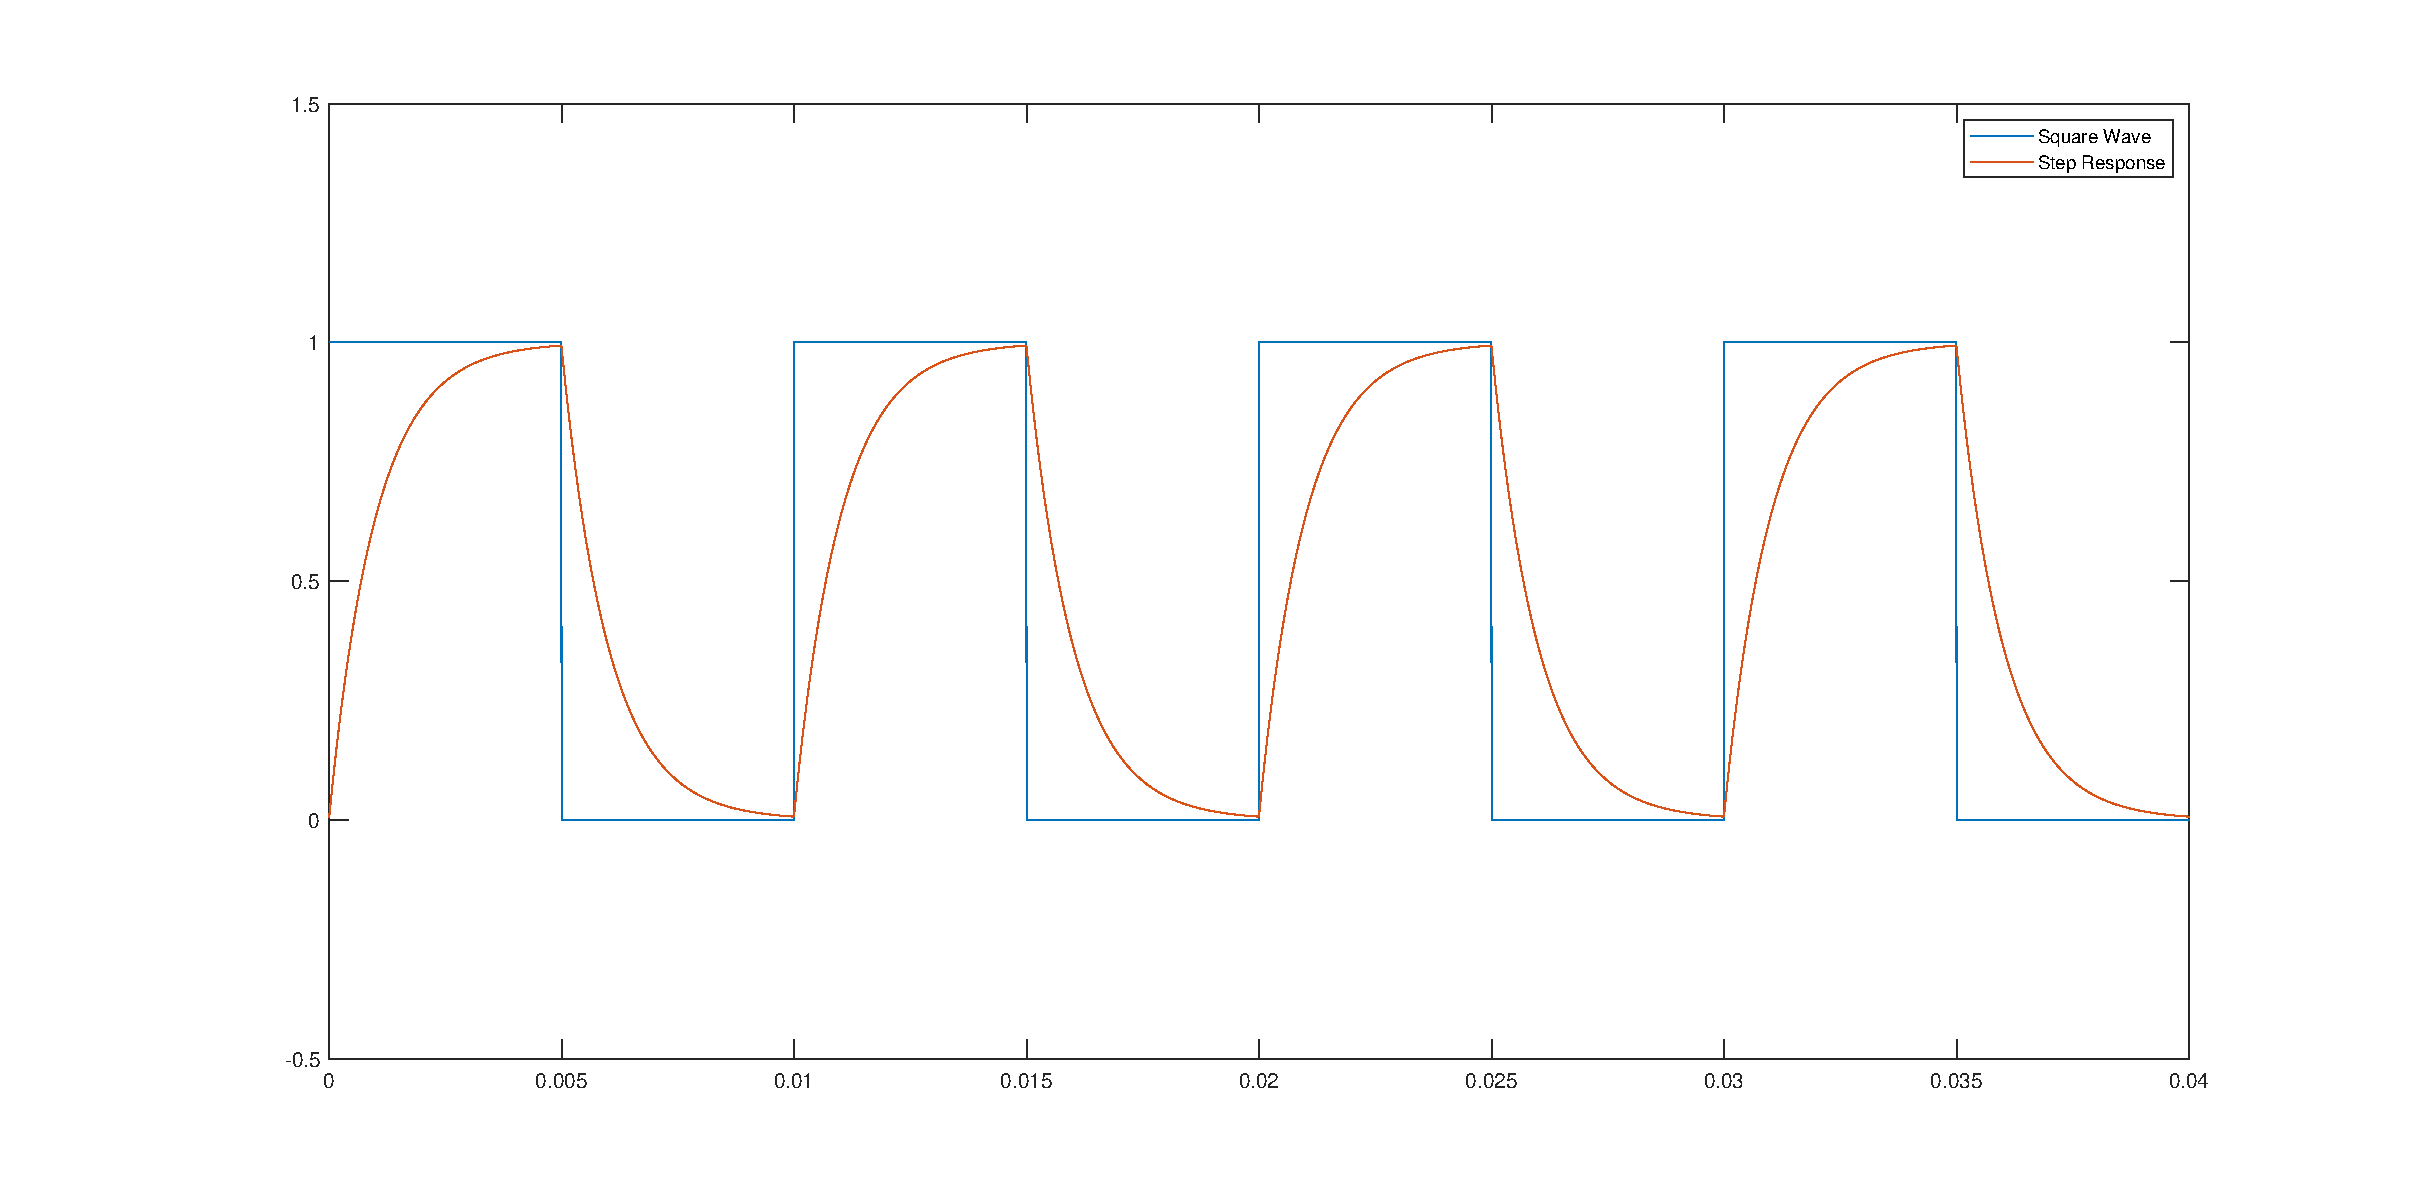
\includegraphics[width=0.8\linewidth]{6.eps}
	\caption{Ideal case of step response.}
\end{figure}
From the graph we find that in the experiment, there is unsmoothness at the rising and falling edge of the square wave shown in Figure 2, while the ideal grave is smooth. It may because the oscilloscope of Proteus intentionally introduces imperfections in the generated square wave signal. However, generally, the shapes of the experimental graph and the ideal graph are very similar.
\subsection{Pulse Response}
In the experiment, we generate pulse waves with a certain width to simulate the dirac delta function. By generating pulse waves with different widths, we can compare them to see the trend of the pulse response as the width becomes smaller. The smaller the width is, the closer the experimental response is to the ideal pulse response.

The ideal cases of the pulse responses with different widths are shown in Figure 7 and Figure 8 respectively.
\begin{figure}[H]
	\centering
	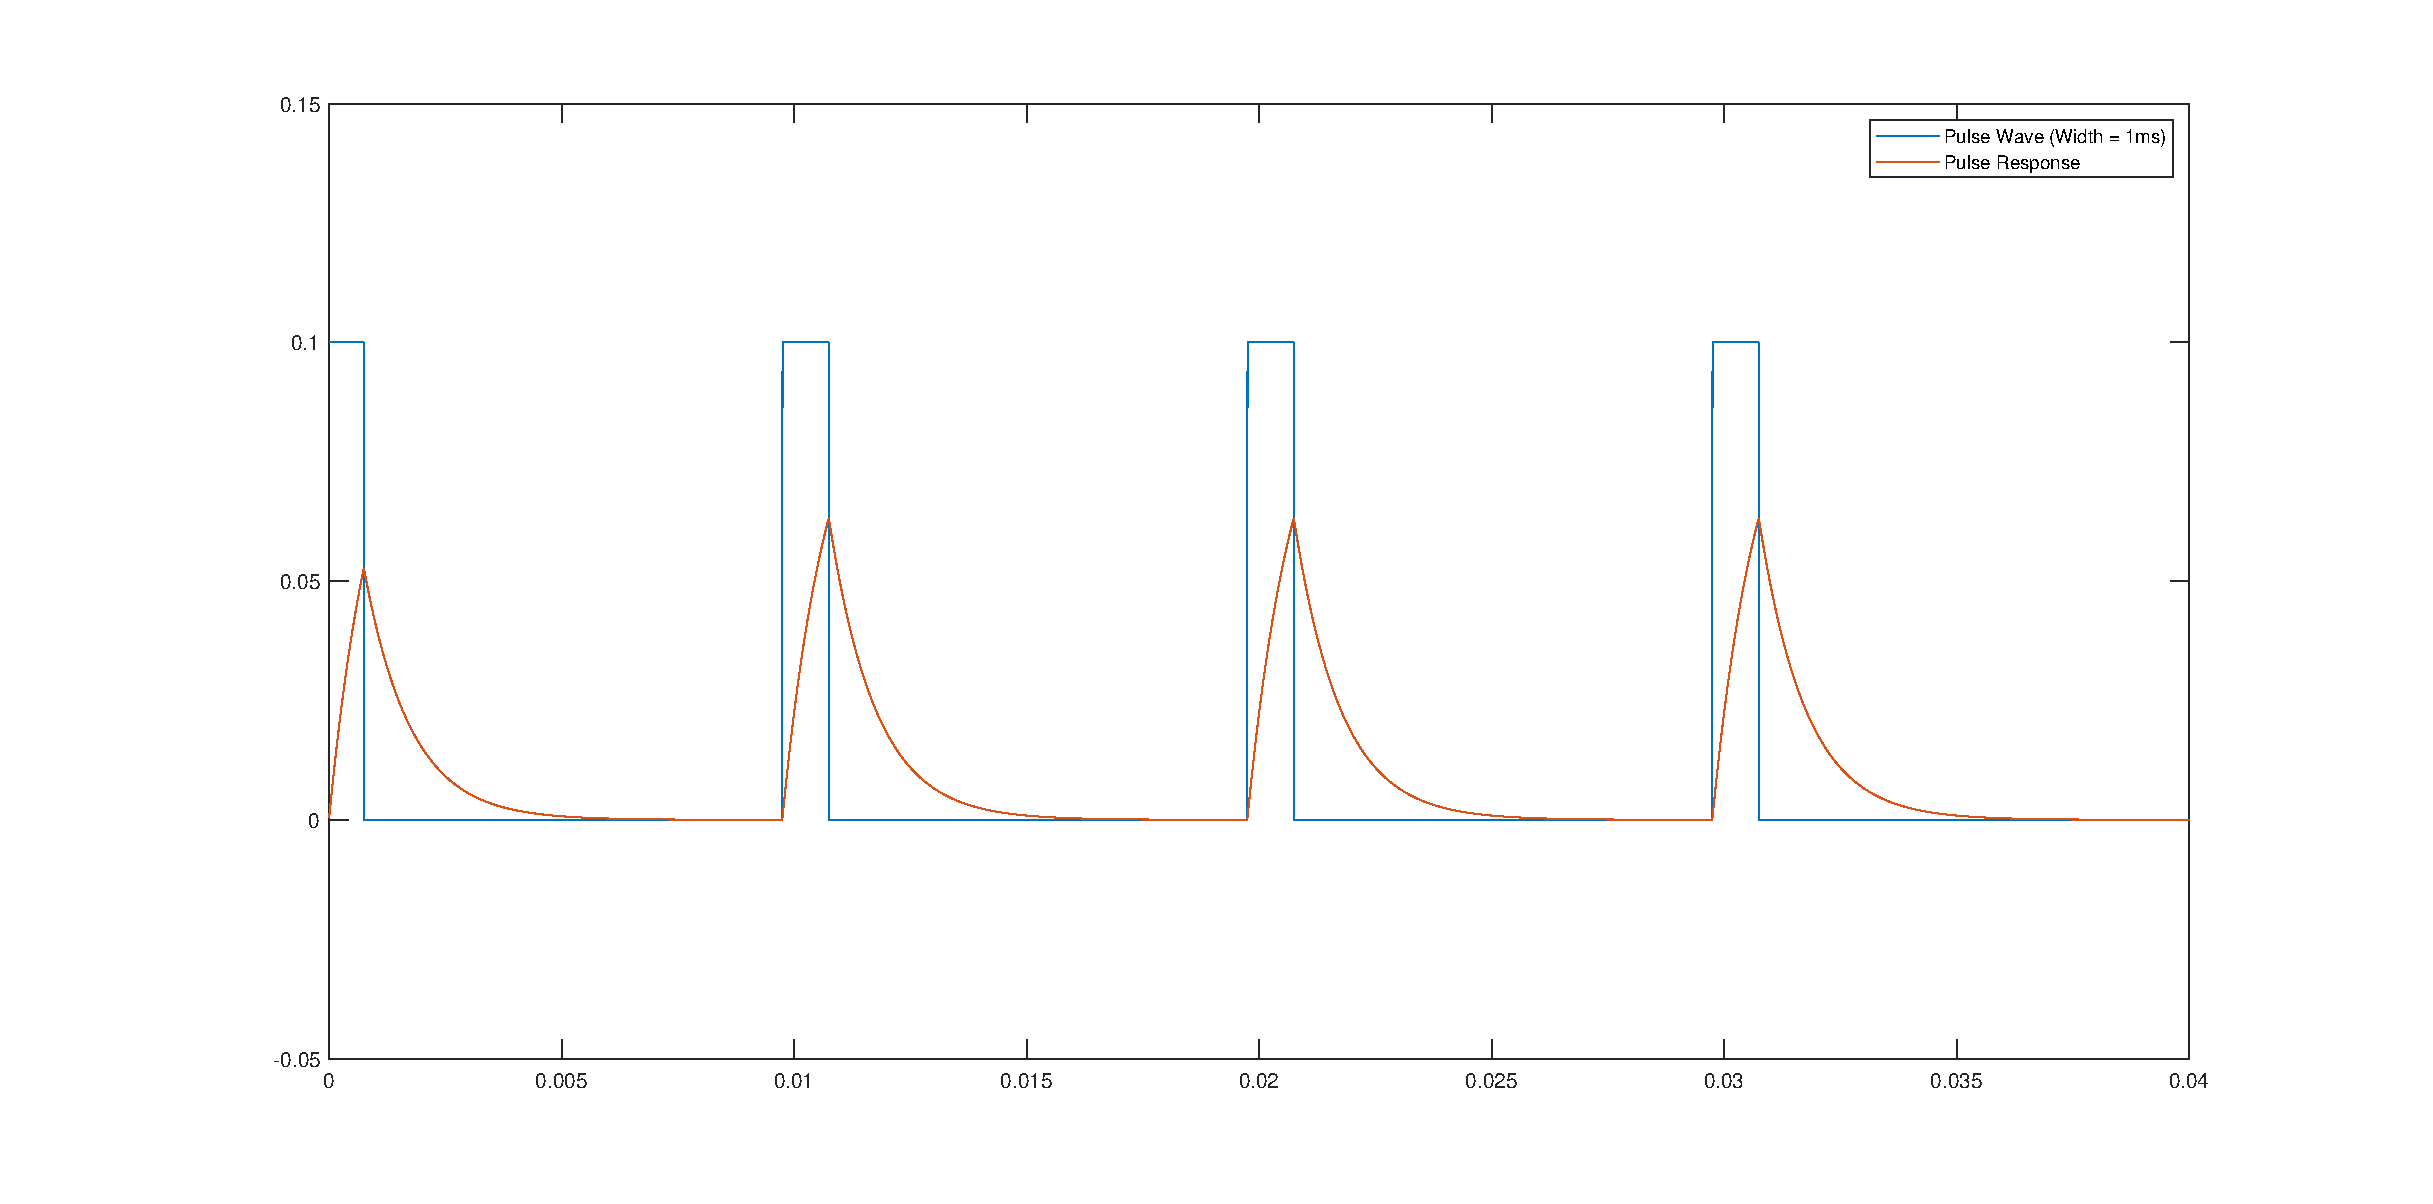
\includegraphics[width=0.8\linewidth]{9.eps}
	\caption{Ideal Pulse Response for width: 1ms, amplitude: 100mV.}
\end{figure}
\begin{figure}[H]
	\centering
	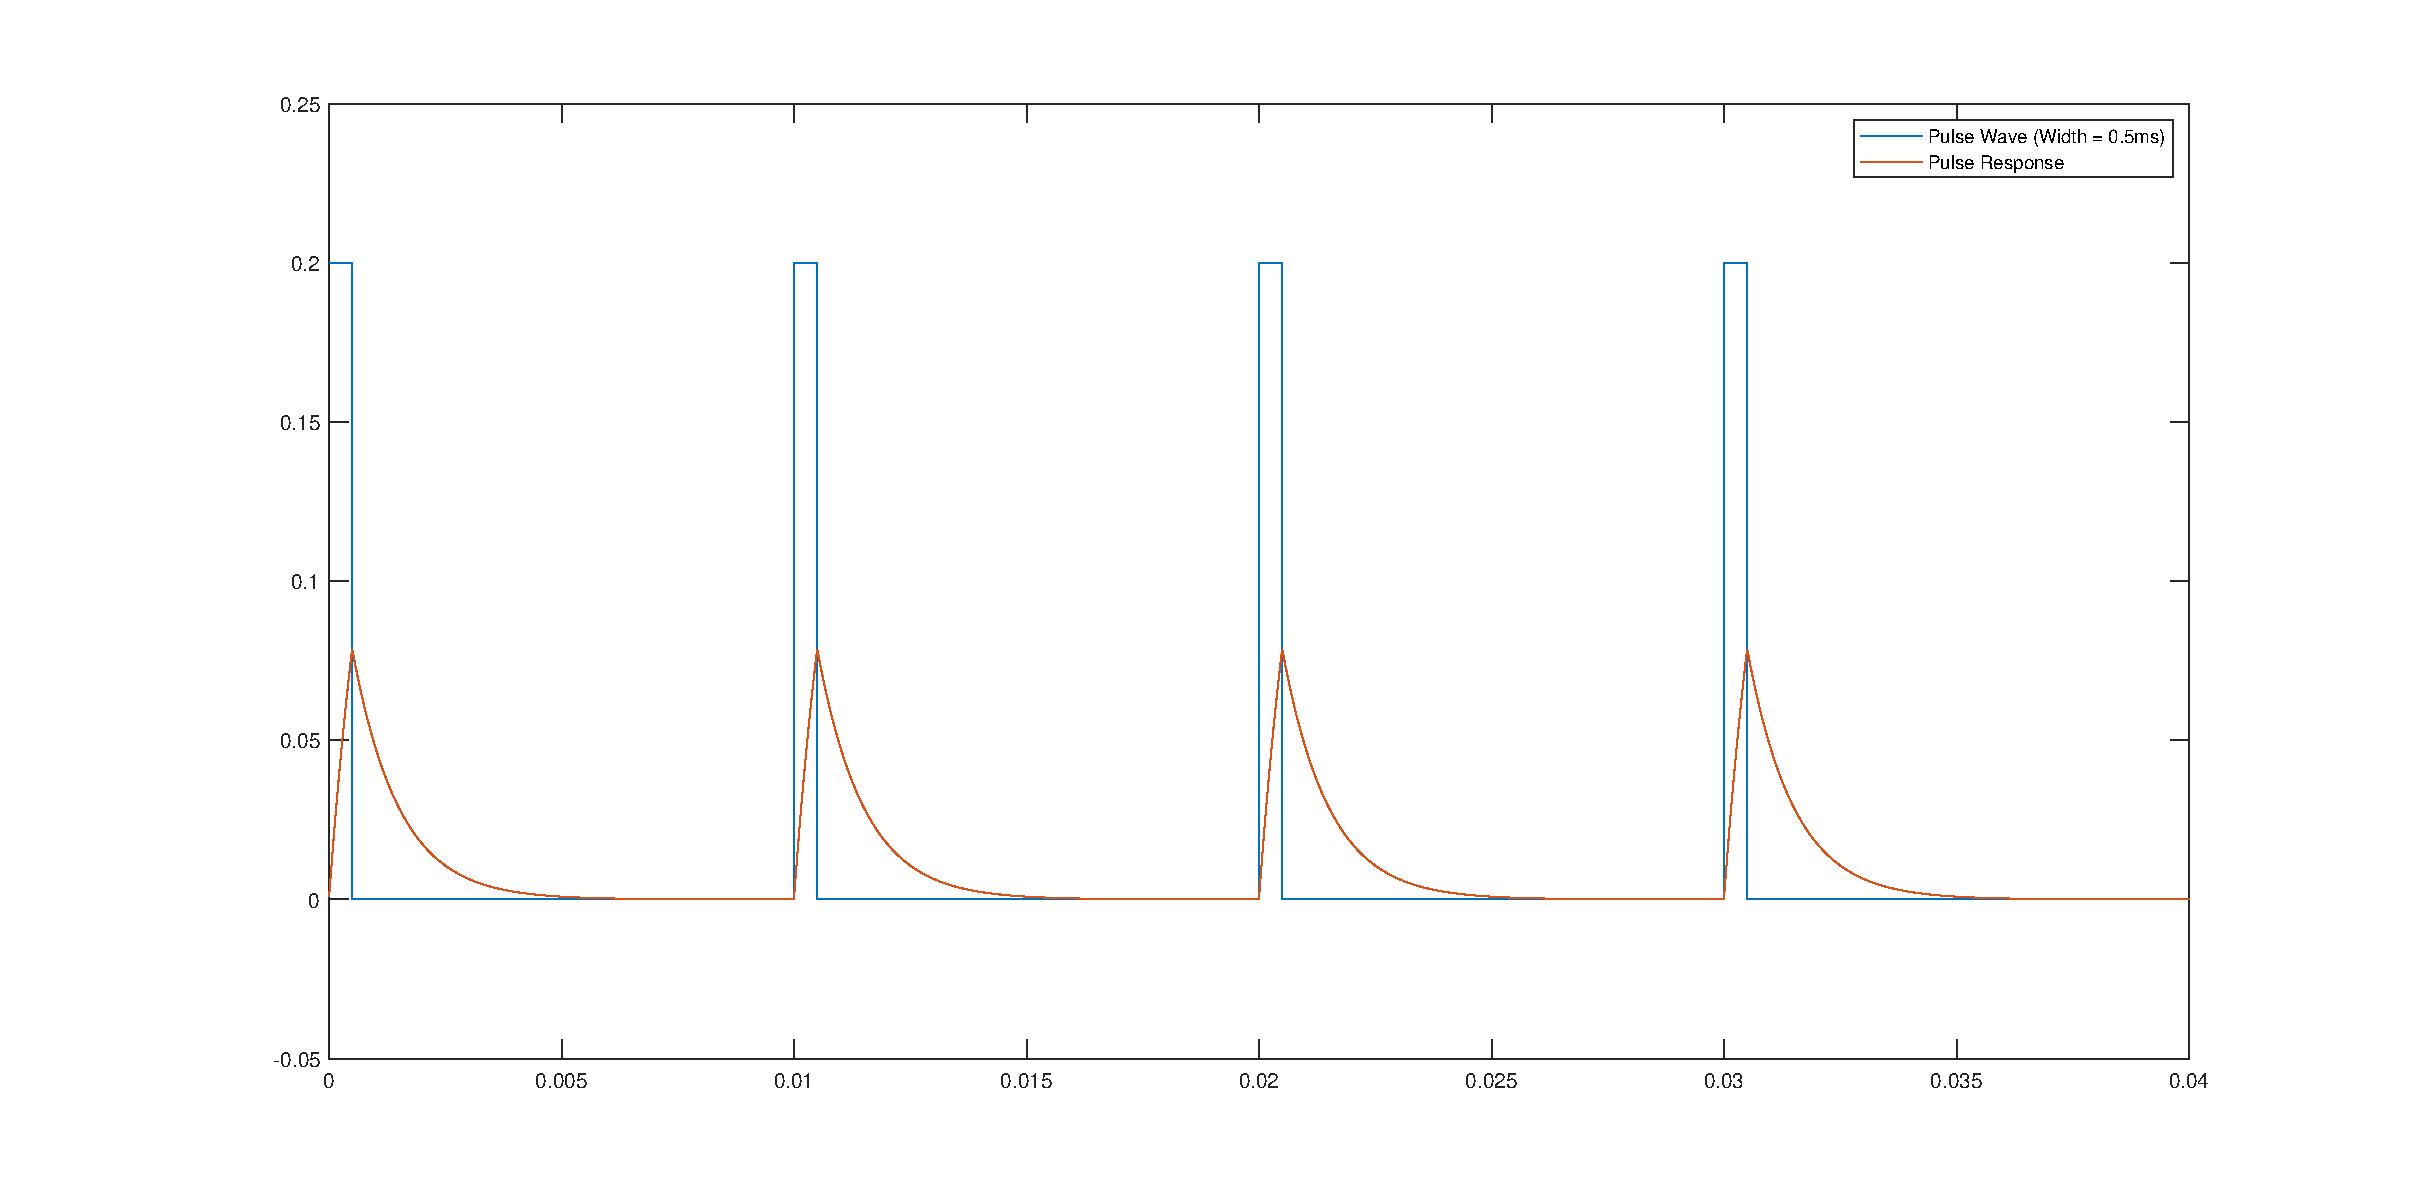
\includegraphics[width=0.8\linewidth]{10.eps}
	\caption{Ideal Pulse Response for width: 0.5ms, amplitude: 200mV.}
\end{figure}
Generally, the shapes of the experimental graph and the ideal graph are very similar.

From prelab we have already derived that the impulse response of the system is
$$h(t)=\frac{\mathrm{d}y_\text{step}(t)}{\mathrm{d}t}=\frac{1}{RC}e^{-t/RC}u(t)$$
The ideal impulse response of the system is shown in Figure 9.
\begin{figure}[H]
	\centering
	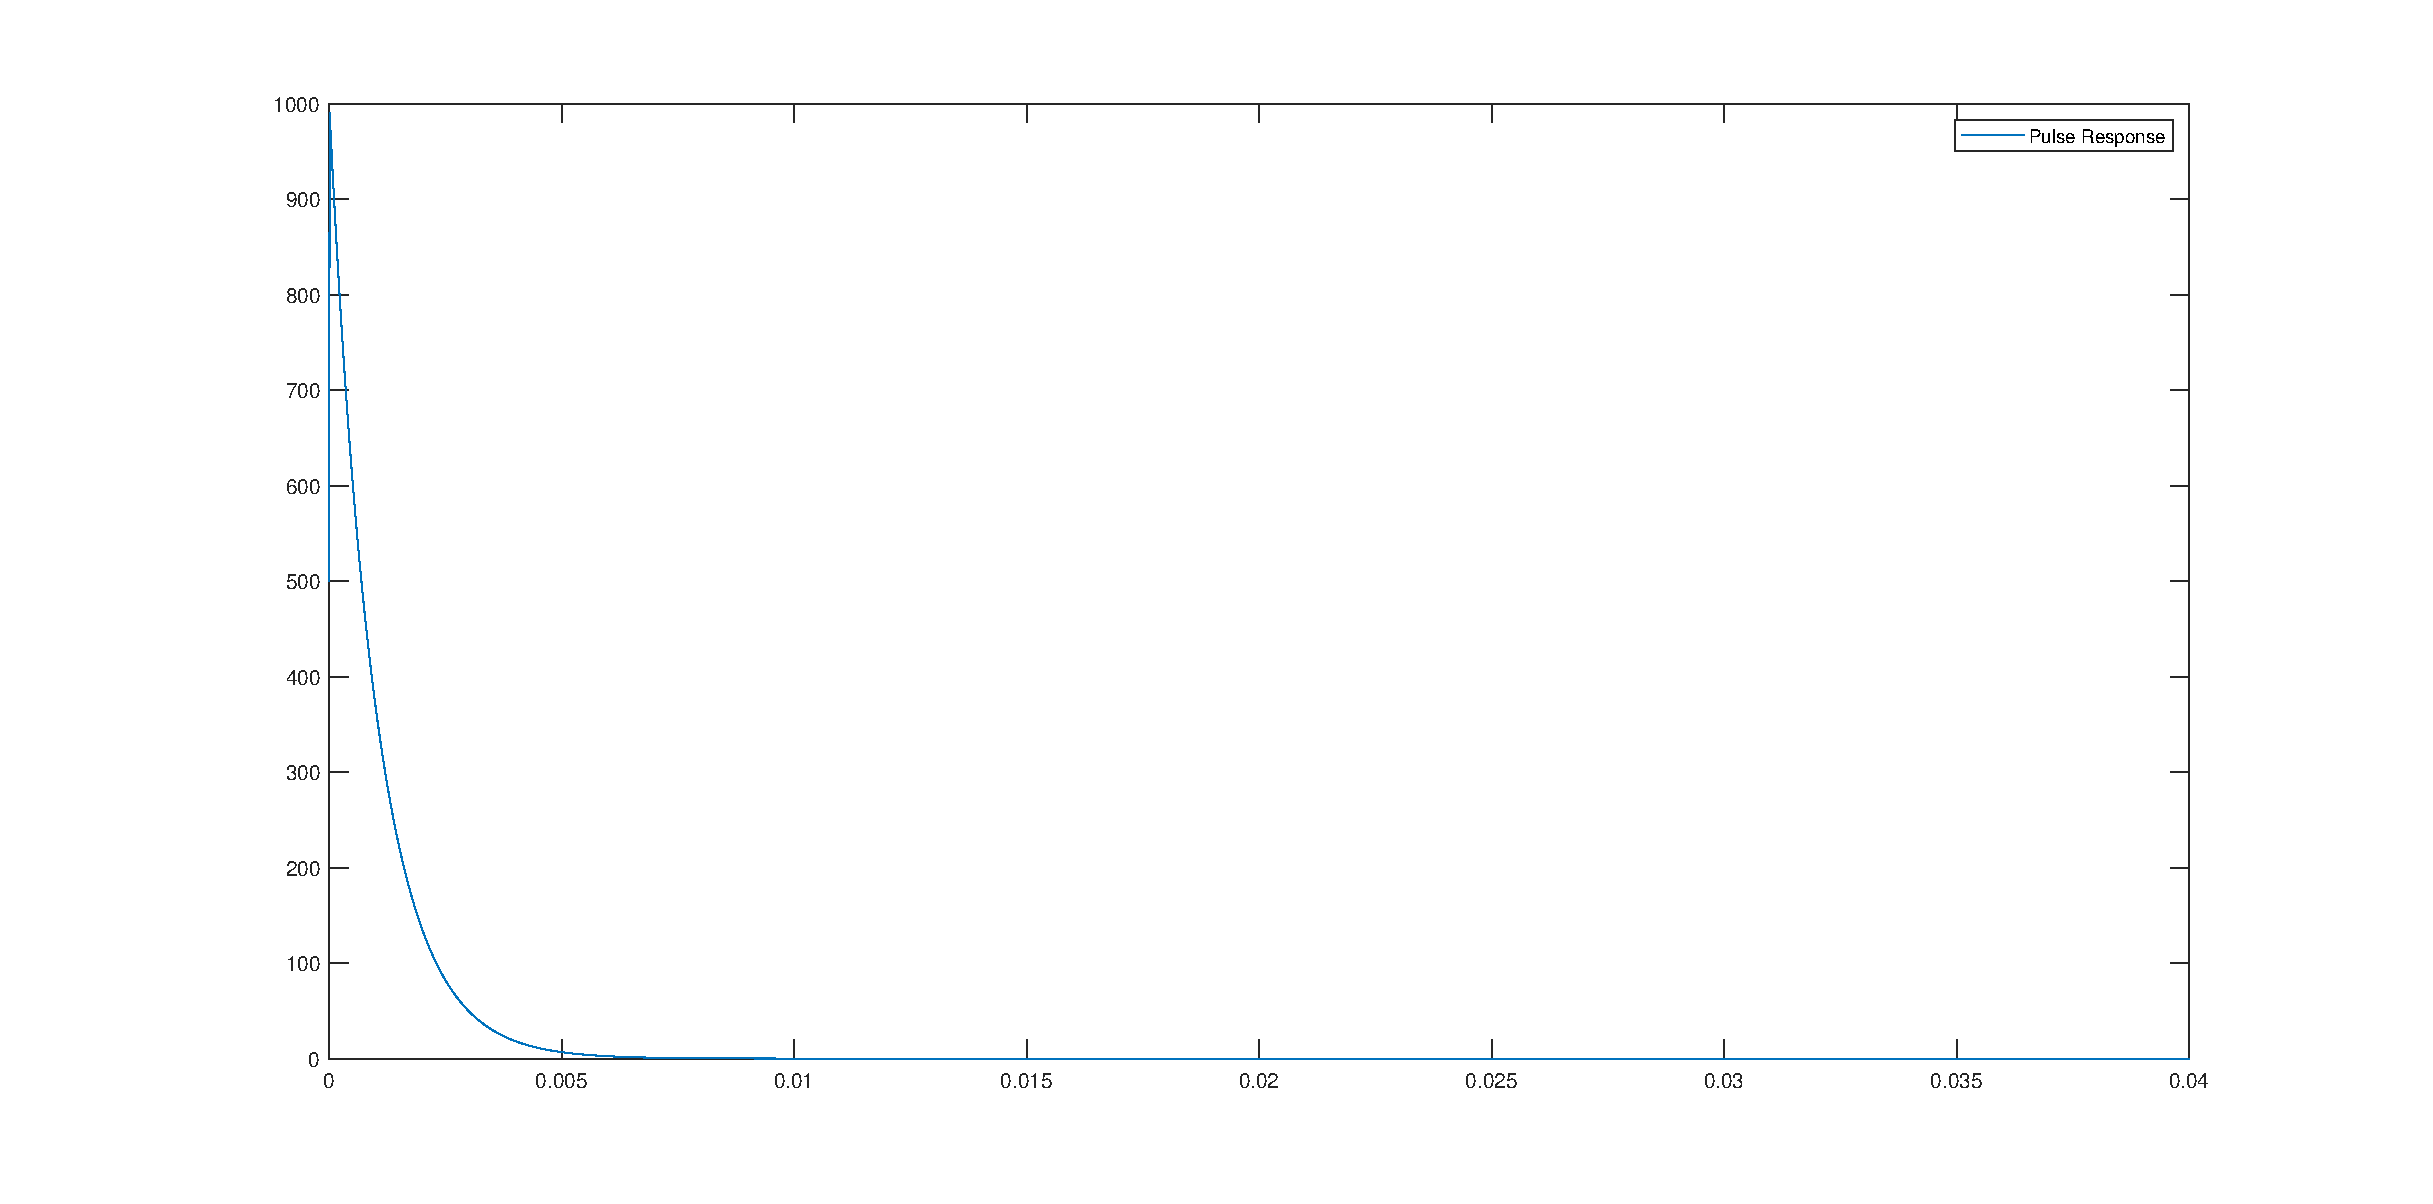
\includegraphics[width=0.8\linewidth]{8.eps}
	\caption{Ideal graph of pulse response.}
\end{figure}
Since it is impossible to really plot an impulse response by vector discrete convolution, we plot the graph of the impulse response $h(t)$. As is shown in the graph, the shape of the graph follows the trend as the width reaches 0.
\subsection{Ramp Response}
In the experiment, due to the limit of Proteus, we use only the right triangular wave to represent the ramp wave. The expression for the wave and its response are respectively
$$x(t)=10(t-0.005)$$
$$y(t)=x(t)*h(t)$$
The ideal graph of the ramp response is shown in Figure 10.
\begin{figure}[H]
	\centering
	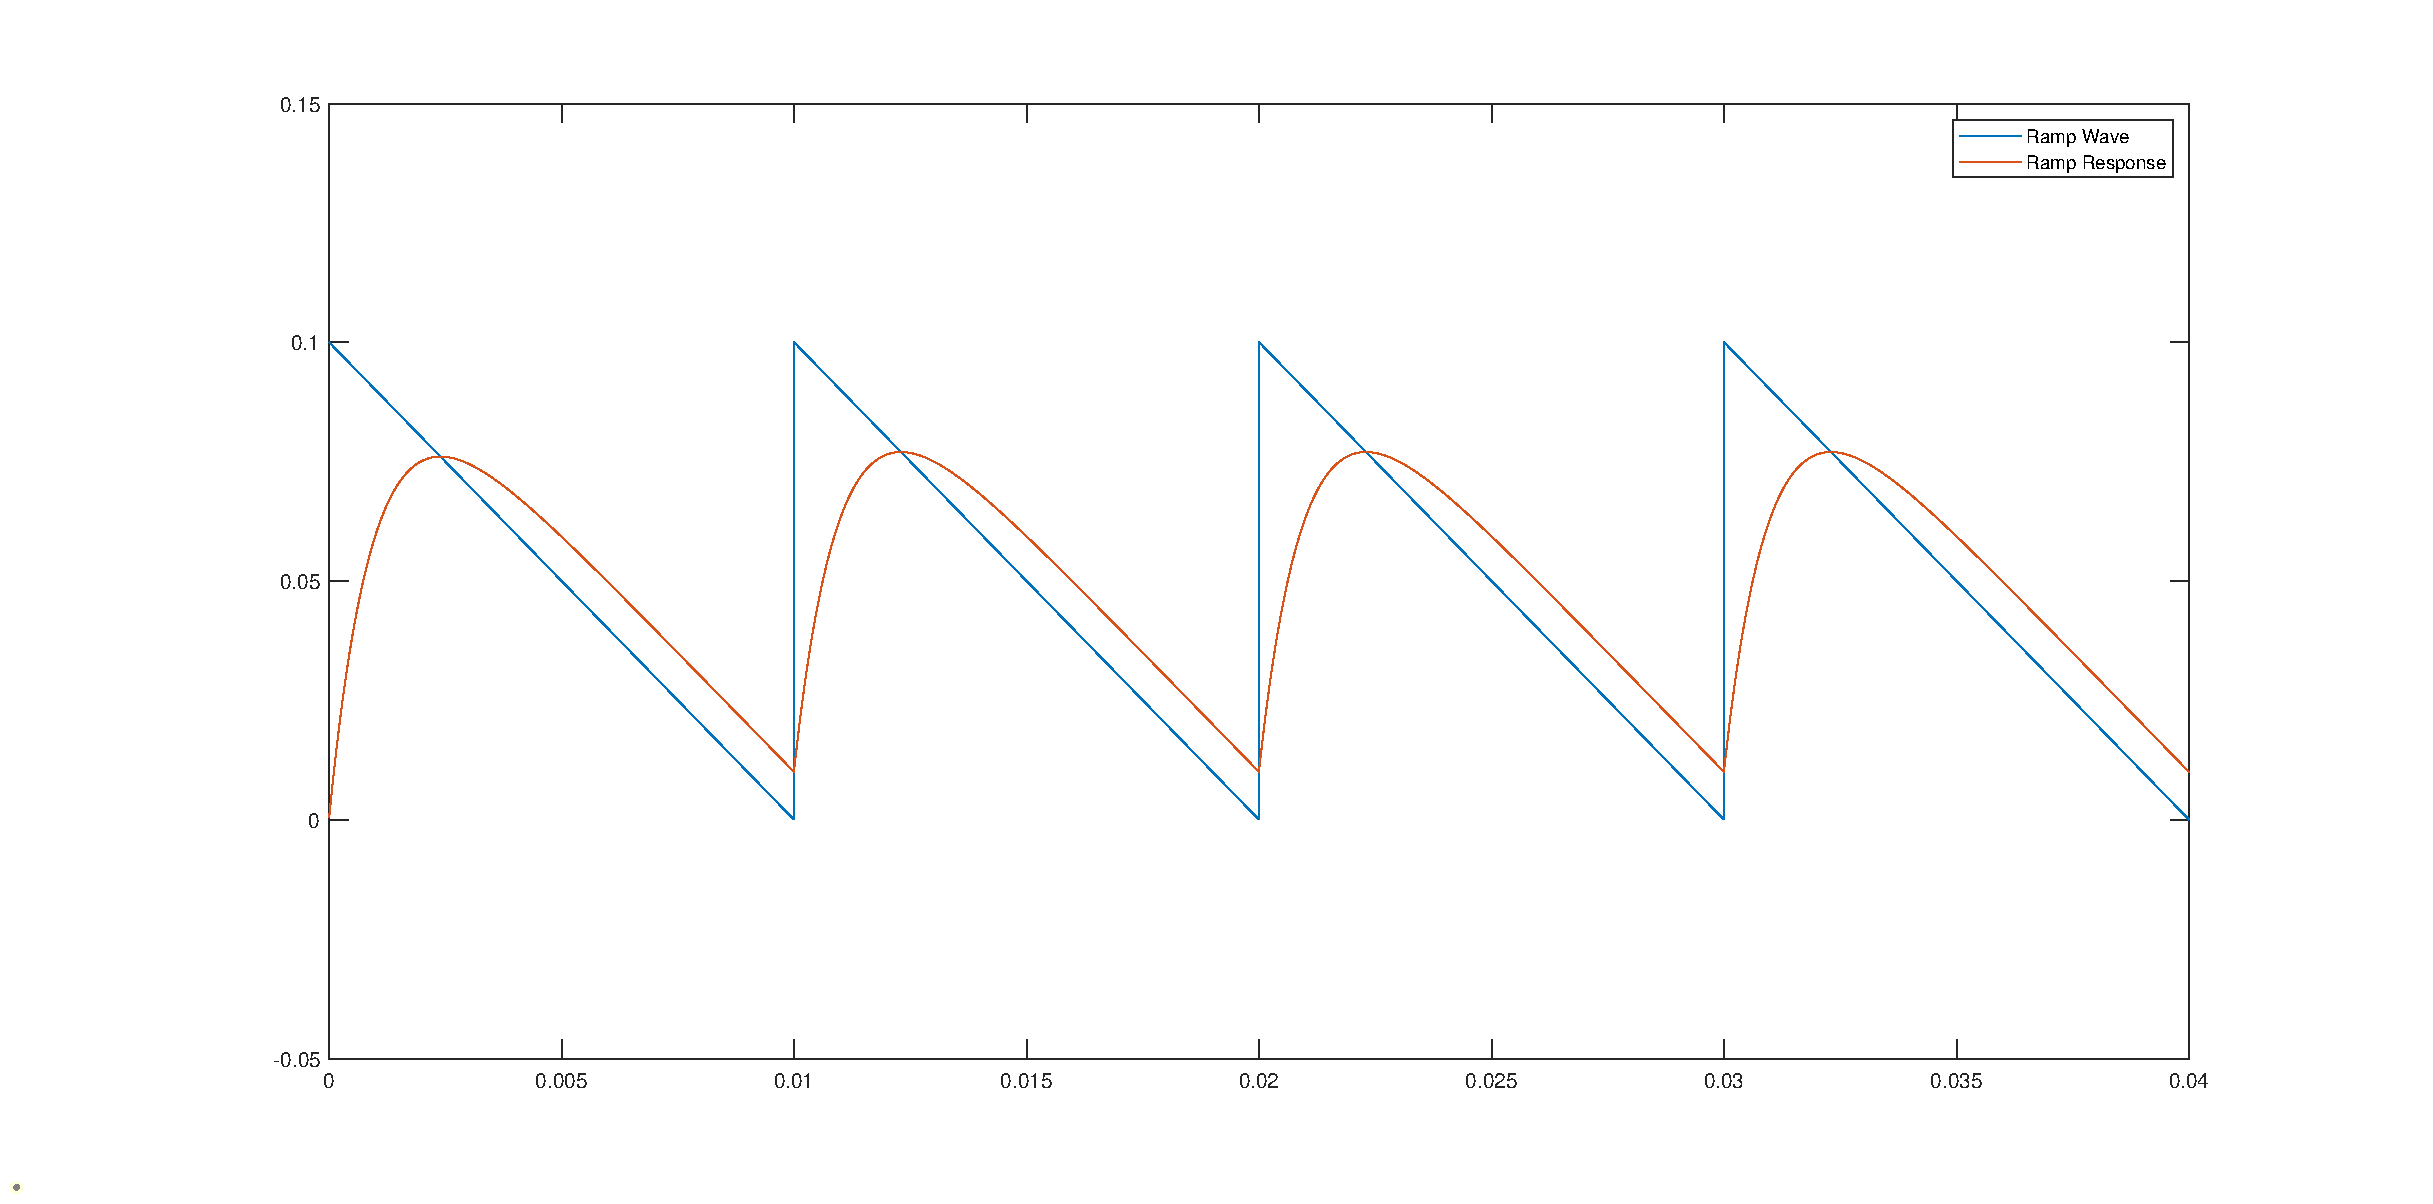
\includegraphics[width=0.7\linewidth]{7.eps}
	\caption{Ideal graph of ramp response}
\end{figure}
From the graph we can see that the shapes of the experimental graph and the ideal graph are very similar.
\subsection{Sine Response}
From prelab we have derived the expressions for the frequency, the time shift, and the phase shift that
$$|H(j2\pi f_c)|=\sqrt{1+(2\pi f_cRC)^2}$$
$$\tau_d=\frac{\arctan(2\pi f_cRC)}{2\pi f_cRC}$$
$$\angle(H(j2\pi f_c))=-\arctan(2\pi f_cRC)$$
Using the formulas above we can calculate the theoretical value as is listed in Table 2.
\begin{table}[H]
	\centering
	\begin{tabular}{|c|c|c|c|}
		\hline
		Frequency (Hz)&$V_\text{out}$ / $V_\text{in}$&Time Shift ($\rm{ms}$)&Phase Shift ($^\circ$)\\
		\hline
		50&0.9540&0.9689&-17.4406\\
		\hline
		500&0.3033&0.4019&-72.3432\\
		\hline
		5k&0.0318&0.0490&-88.1768\\
		\hline
	\end{tabular}
	\caption{Theoretical values of the sine response.}
\end{table}
Using the data from Table 1 and Table 2, we can derive the errors in Table 3 and the relative errors in Table 4.
\begin{table}[H]
	\centering
	\begin{tabular}{|c|c|c|c|}
		\hline
		Frequency (Hz)&$V_\text{out}$ / $V_\text{in}$&Time Shift ($\rm{ms}$)&Phase Shift ($^\circ$)\\
		\hline
		50&0.004&0.03&0.6\\
		\hline
		500&0.003&0.001&0.3\\
		\hline
		5k&0.0002&0.0010&1.8\\
		\hline
	\end{tabular}
	\caption{Errors of the sine response.}
\end{table}
\begin{table}[H]
	\centering
	\begin{tabular}{|c|c|c|c|}
		\hline
		Frequency (Hz)&$V_\text{out}$ / $V_\text{in}$&Time Shift&Phase Shift\\
		\hline
		50&0.4\%&3.2\%&3.2\% \\
		\hline
		500&1.1\%&0.5\%&0.5\%\\
		\hline
		5k&0.6\%&2.0\%&2.0\%\\
		\hline
	\end{tabular}
	\caption{Relative errors of the sine response.}
\end{table}
The errors of the time shift and the phase shift when $f=50\rm{Hz}$ is a little larger than others which is possibly because the scale of the oscilloscope when reading is not small enough to read very accurate values.
\section{Conclusion}
During the experimental, we generally achieves our goals.

When drawing schematics, we became more familiar with instruments including different signal generators, oscilloscope, and virtual electric components and reviewed the knowledge we learned from VE215 course. Besides, we used the knowledge of different signals learned in VE216 signal and system course.

To derive the output signal of an LTI system or response when the input signal is a step, pulse, ramp, or sine signal, we used the properties of an LTI system. Based on that, we compared the experimental and the ideal results of different cases.

In part Step Response, we compared the graphs and found that there is unsmoothness at the rising and falling edge of the square wave shown in Figure 2, while the ideal grave is smooth. It may because the oscilloscope of Proteus intentionally introduces imperfections in the generated square wave signal.

In part Pulse Response, we compared the graphs of different widths of the pulse wave and concluded that as the width reaches 0 the pulse response will reaches the impulse response of the system.

In part Ramp Response, we compared the graphs and found that the experimental graphs fits the ideal graphs generated by vector convolution.

In part Sine Response, we read the values of $V_\text{out}$, $V_\text{in}$, and the time shift and calculated the ratio of $V_\text{out}$ and $V_\text{in}$ and the phase shift. Then we compared them with the theoretical values and calculate the errors and relative errors. The errors are possibly resulted from the limited time scale and the voltage scale when reading the values.
\section{Appendices}
\subsection{MATLAB Code}
\lstinputlisting{Lab1.m}
\subsection{References}
\begin{enumerate}
	\item Lab 1: LTI Systems Part I: Intro \& Pre-lab Assignment Borrowed from UMich EECS 216.
	\item Lab1 Manual.
\end{enumerate}
\end{document}